\subsubsection{UserController}
\begin{figure}[h]
\centering
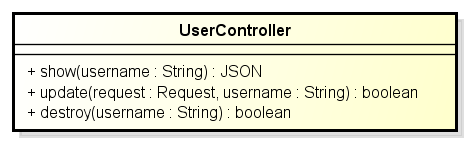
\includegraphics[width=0.8\linewidth]{img/back_end_http_controllers_userController}
\caption[Diagramma della classe UserController]{Diagramma della classe UserController}
\label{fig:back_end_http_controllers_userController}
\end{figure}

	\paragraph{Descrizione}
		Questa classe gestisce i dati dell'utente sfruttando i dati forniti dal model.
	\paragraph{Utilizzo}
		La classe è progettata per consentire l'interrogazione, la manipolazione e l'eliminazione dei dati dell'utente.

	\paragraph{Metodi}
		\begin{itemize}
			\item \textbf{+ show(username: String) : JSON}\\
			Il metodo verifica se c'è un utente autenticato. Se la verifica ha avuto successo si procede con il recupero dei dati dell'utente a cui corrisponde la variabile \textit{username}, in particolare il suo profilo, e restituisce un oggetto \gls{JSON} contenente tali informazioni:\\
			\textbf{Argomenti}
			\begin{itemize}
				\item username : String;\\
				Stringa contenente il nome utente.
			\end{itemize}
			
			\newpage
			\item \textbf{+ update(request: Request, username: String) : boolean}\\
			Il metodo recupera l'utente autenticato e aggiorna i dati del profilo contenuti nella richiesta HTTP \textit{request}. Il metodo ritorna un valore booleano che indica che i dati sono stati aggiornati:\\
			\textbf{Argomenti}
			\begin{itemize}
				\item request : Request;\\
				Richiesta HTTP contenente i valori con cui eseguire l'aggiornamento del profilo utente.
				\item username : String;\\
				Stringa contenente il nome utente.
			\end{itemize}
			
			\item \textbf{+ destroy(username: String) : boolean}
			Il metodo recupera l'utente autenticato e lo cancella dal \gls{database} insieme a tutte le  sue informazioni. Il metodo ritorna un valore booleano che indica l'avvenuta cancellazione dal \gls{database}:\\
			\textbf{Argomenti}
			\begin{itemize}
				\item username : String;\\
				Stringa contenente il nome utente.
			\end{itemize}
		\end{itemize}
		
\newpage
\subsubsection{ProjectController}
\begin{figure}[h]
\centering
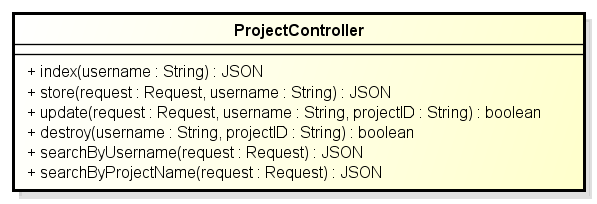
\includegraphics[width=0.8\linewidth]{img/back_end_http_controllers_projectController}
\caption[Diagramma della classe ProjectController]{Diagramma della classe ProjectController}
\label{fig:back_end_http_controllers_projectController}
\end{figure}

	\paragraph{Descrizione}
		Questa classe gestisce i dati di un progetto.
	\paragraph{Utilizzo}
		La classe è progettata per consentire la creazione, la manipolazione dei dati, l'interrogazione e l'eliminazione di un progetto.
		
	\paragraph{Metodi}
		\begin{itemize}
			\item \textbf{+ index(username: String) : JSON}\\
			Il metodo recupera tutti i progetti dell'utente autenticato e li restituisce. Il metodo restituisce un oggetto \gls{JSON} con le informazioni richieste:\\
			\textbf{Argomenti}
			\begin{itemize}
				\item username : String;\\
				Stringa contenente il nome utente.
			\end{itemize}
			
			\item \textbf{+ store(request: Request, username: String) : boolean}\\
			Il metodo crea un nuovo progetto assegnandoli un nome e lo salva nel \gls{database} all'interno della collection relativa all'utente autenticato. Il metodo restituisce un oggetto \gls{JSON} contenente il progetto appena creato. Inoltre emette un segnale di tipo \textit{ProjectWasCreated} per la corretta inizializzazione della presentazione relativa al nuovo progetto:\\
			\textbf{Argomenti}
			\begin{itemize}
				\item request : Request;\\
			 	Richiesta HTTP contenente i valori con cui eseguire la creazione del progetto.
			 	\item username : String;\\
			 	Stringa contenente il nome utente.
			\end{itemize}
			
			\item \textbf{+ update(request: Request, username: String, projectID: String) : boolean}\\
			Il metodo recupera il progetto dell'utente autenticato tramite projectID ed aggiorna i dati del progetto. Il metodo ritorna un valore booleano che indica che l'aggiornamento delle informazioni è avvenuto:\\
			\textbf{Argomenti}
			\begin{itemize}
				\item request : Request;\\
				Richiesta HTTP contenente i valori con cui eseguire l'aggiornamento dei dati del progetto.
				\item username : String;\\
				Stringa contenente il nome utente.
				\item projectID : string; \\
				Stringa contenente l'ID univoco di un progetto.
			\end{itemize}
			
			\item \textbf{+ destroy(username: String, projectID: String) : boolean}\\
			Il metodo recupera il progetto dell'utente autenticato, indicato da projectID, e lo cancella dal \gls{database} insieme a tutte le sue informazioni. Il metodo ritorna un valore booleano che indica che la cancellazione del progetto dal \gls{database} è avvenuta:\\
			\textbf{Argomenti}
			\begin{itemize}
				\item username : String;\\
				Stringa contenente il nome utente.
				\item projectID : string; \\
				Stringa contenente l'ID univoco di un progetto.
			\end{itemize}
			
			\item \textbf{+ searchByUsername(request: Request) : JSON}\\
			Il metodo ritorna un oggetto \gls{JSON} contenente la lista di tutti gli utenti che hanno \textit{username} uguale a quello inserito nell'apposito form:\\
			\textbf{Argomenti}
			\begin{itemize}
				\item request : Request;\\
				Richiesta HTTP contenente il valore con cui effettuare la ricerca.
			\end{itemize}
			
			\item \textbf{+ searchByProjectName(request: Request) : JSON}\\
			Il metodo ritorna un oggetto \gls{JSON} contenente la lista di tutti i progetti che hanno \textit{name} uguale a quello inserito nell'apposito form:\\
			\textbf{Argomenti}
			\begin{itemize}
				\item request : Request;\\
				Richiesta HTTP contenente il valore con cui effettuare la ricerca.
			\end{itemize}
		\end{itemize}
		
\newpage
\subsubsection{InfographicController}
\begin{figure}[h]
\centering
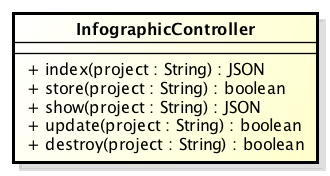
\includegraphics[width=0.8\linewidth]{img/back_end_http_controllers_infographicController}
\caption[Diagramma della classe InfographicController]{Diagramma della classe InfographicController}
\label{fig:back_end_http_controllers_infographicController}
\end{figure}

	\paragraph{Descrizione}
		Questa classe gestisce i dati di un'\gls{infografica}.
	\paragraph{Utilizzo}
		La classe è progettata per consentire la creazione, la manipolazione dei dati, l'interrogazione e l'eliminazione di un'\gls{infografica}.
		
	\paragraph{Metodi}
		\begin{itemize}
			\item \textbf{+ index(username: String, projectID: String) : JSON}\\
			Il metodo recupera le infografiche relative ad un progetto dell'utente autenticato e restituisce un oggetto \gls{JSON} con tutte le infografiche associate al progetto:\\
			\textbf{Argomenti}
			\begin{itemize}
				\item username : String; \\
				Stringa contenente il nome utente.
				\item projectID : String; \\
				Stringa contenente l'ID univoco di un progetto associato all'utente autenticato.
			\end{itemize}
			
			\item \textbf{+ store(request: Request, username: String, projectID: String) : JSON}\\
			Il metodo crea una nuova \gls{infografica} assegnandoli un nome e il path per il salvataggio e la salva nel progetto con ID = projectID relativo all'utente autenticato. Il metodo ritorna un oggetto \gls{JSON} contenente l'\gls{infografica} appena creata:\\
			\textbf{Argomenti}
			\begin{itemize}
				\item request : Request;\\
				Richiesta HTTP contenente i valori con cui creare l'\gls{infografica}.
				\item username : String; \\
				Stringa contenente il nome utente.
				\item projectID : String; \\
				Stringa contenente l'ID univoco di un progetto associato all'utente autenticato.
			\end{itemize}
			
			\item \textbf{+ show(username: String, projectID: String, infographicID: String) : JSON}\\
			Il metodo interroga il \gls{database} recuperando il progetto con l'ID = projectID relativo all'utente autenticato ed a partire dal progetto recupera l'\gls{infografica} con ID = infographicID. Il metodo ritorna un oggetto \gls{JSON} con le informazioni richieste dell'\gls{infografica}:\\
			\textbf{Argomenti}
			\begin{itemize}
				\item username : String; \\
				Stringa contenente il nome utente.
				\item projectID : String; \\
				Stringa contenente l'ID univoco di un progetto associato all'utente autenticato.
				\item infographicID : String; \\
				Stringa contenente l'ID univoco di un'\gls{infografica} associato al progetto.
			\end{itemize}
			
			\item \textbf{+ update(request: Request, username: String, projectID: String, infographicID: String) : boolean}\\
			Il metodo recupera il progetto con ID = projectID relativo all'utente autenticato ed a partire dal progetto recupera l'\gls{infografica} con ID = infographicID ed aggiorna i dati \textit{name} e \textit{path} dell'\gls{infografica}. Il metodo ritorna un valore booleano che indica che l'aggiornamento è stato effettuato:\\
			\textbf{Argomenti}
			\begin{itemize}
				\item request : Request;\\
				Richiesta HTTP contenente i valori con cui aggiornare l'\gls{infografica}.
				\item username : String; \\
				Stringa contenente il nome utente.
				\item projectID : String; \\
				Stringa contenente l'ID univoco di un progetto associato all'utente autenticato.
				\item infographicID : String; \\
				Stringa contenente l'ID univoco di un'\gls{infografica} associato al progetto.
			\end{itemize}
			
			\item \textbf{+ destroy(username: String, projectID: String, infographicID: String) : boolean}\\
			Il metodo recupera il progetto con ID = projectID relativo all'utente autenticato ed a partire dal progetto recupera l'\gls{infografica} con ID = infographicID chiamando il metodo \textit{delete} su tale \gls{infografica} cancellandola dal \gls{database}. Il metodo ritorna un valore booleano che indica che la cancellazione è avvenuta:\\
			\textbf{Argomenti}
			\begin{itemize}
				\item username : String; \\
				Stringa contenente il nome utente.
				\item projectID : String; \\
				Stringa contenente l'ID univoco di un progetto associato all'utente autenticato.
				\item infographicID : String; \\
				Stringa contenente l'ID univoco di un'\gls{infografica} associato al progetto.
			\end{itemize}
		\end{itemize}
		
\newpage
\subsubsection{PresentationController}
\begin{figure}[h]
\centering
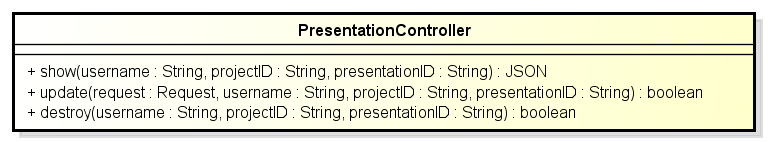
\includegraphics[width=0.8\linewidth]{img/back_end_http_controllers_presentationController}
\caption[Diagramma della classe PresentationController]{Diagramma della classe PresentationController}
\end{figure}


	\paragraph{Descrizione}
		Questa classe gestisce i dati della presentazione.
	\paragraph{Utilizzo}
		La classe è stata progettata per consentire l'interrogazione, la manipolazione dei dati e l'eliminazione di una presentazione.
	
	\paragraph{Metodi}
		\begin{itemize}
			\item \textbf{+ show(username: String, projectID: String, presentationID: String) : JSON}\\
			Il metodo interroga il \gls{database} recuperando il progetto con l'ID = projectID relativo all'utente autenticato ed a partire dal progetto recupera la presentazione con ID = presentationID. Il metodo ritorna un oggetto \gls{JSON} con le informazioni richieste della presentazione:\\
			\textbf{Argomenti}
			\begin{itemize}
				\item username : String; \\
				Stringa contenente il nome utente.
				\item projectID : String; \\
				Stringa contenente l'ID univoco di un progetto associato all'utente autenticato.
				\item presentationID : String; \\
				Stringa contenente l'ID univoco della presentazione associata al progetto.
			\end{itemize}
			
			\item \textbf{+ update(request: Request, username: String, projectID: String, presentationID: String) : boolean}\\
			Il metodo recupera il progetto con ID = projectID relativo all'utente autenticato ed a partire dal progetto recupera la presentazione con ID = presentationID ed aggiorna i dati \textit{theme} e \textit{transition} della presentazione. Il metodo ritorna un valore booleano che indica che l'aggiornamento è stato effettuato:\\
			\textbf{Argomenti}
			\begin{itemize}
				\item request : Request;\\
				Richiesta HTTP contenente i valori con cui aggiornare la presentazione.
				\item username : String; \\
				Stringa contenente il nome utente.
				\item projectID : String; \\
				Stringa contenente l'ID univoco di un progetto associato all'utente autenticato.
				\item presentationID : String; \\
				Stringa contenente l'ID univoco di una presentazione associata al progetto.
			\end{itemize}
			\newpage
			\item \textbf{+ destroy(username: String, projectID: String, presentationID: String) : boolean}\\
			Il metodo recupera il progetto con ID = projectID relativo all'utente autenticato ed a partire dal progetto recupera la presentazione con ID = presentationID chiamando il metodo \textit{delete} su tale presentazione cancellandola dal \gls{database}. Il metodo ritorna un valore booleano che indica che la cancellazione è avvenuta:\\
			\textbf{Argomenti}
			\begin{itemize}
				\item username : String; \\
				Stringa contenente il nome utente.
				\item projectID : String; \\
				Stringa contenente l'ID univoco di un progetto associato all'utente autenticato.
				\item presentationID : String; \\
				Stringa contenente l'ID univoco di una presentazione associata al progetto.
			\end{itemize}
		\end{itemize}
		
\newpage
\subsubsection{SlideController}
\begin{figure}[h]
\centering
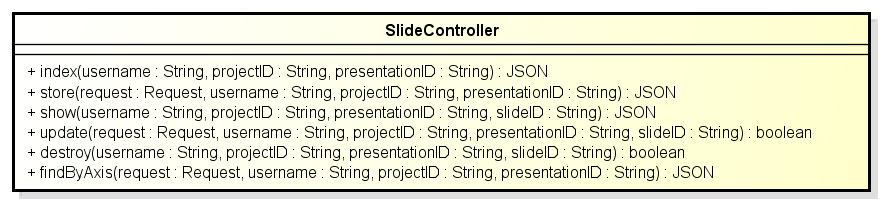
\includegraphics[width=0.8\linewidth]{img/back_end_http_controllers_slideController}
\caption[Diagramma della classe SlideController]{Diagramma della classe SlideController}
\label{fig:back_end_http_controllers_slideController}
\end{figure}

	\paragraph{Descrizione}
		Questa classe gestisce i dati di una \gls{slide}.
	\paragraph{Utilizzo}
		La classe è stata progettata per consentire la creazione e la manipolazione dei dati di una \gls{slide}.

	\paragraph{Metodi}
		\begin{itemize}
			\item \textbf{+ index(username: String, projectID: String, presentationID: String) : \gls{JSON}}\\
				Il metodo recupera il progetto con ID = projectID relativo all'utente autenticato, per poi recuperare l'unica presentazione associata a tale progetto e restituisce tutte le \gls{slide} associate ad essa. Il metodo ritorna un oggetto \gls{JSON} contenente le \gls{slide} all'interno della presentazione:\\
				\textbf{Argomenti:}
				\begin{itemize}
					\item username : String; \\
					Stringa contenente il nome utente.
					\item projectID : String; \\
					Stringa contenente l'ID univoco di un progetto associato all'utente autenticato.
					\item presentationID : String; \\
					Stringa contenente l'ID univoco di una presentazione associata al progetto.
				\end{itemize}
				
			\item \textbf{+ store(request: Request, username: String, projectID: String, presentationID: String) : \gls{JSON}}\\
				Il metodo crea una nuova \gls{slide} recuperando il progetto con ID = projectID relativo all'utente autenticato, per poi recuperare l'unica presentazione associata a tale progetto e la \gls{slide} con ID = slideID. Invoca il metodo statico della classe Presentation \textit{incrementIndex} che aggiorna in modo corretto tutti gli indici delle \gls{slide} della presentazione. Il metodo ritorna un oggetto \gls{JSON} che contiene la \gls{slide} appena creata:\\
				\textbf{Argomenti:}
				\begin{itemize}
					\item request : Request;\\
					Richiesta HTTP contenente i componenti da inserire nella \gls{slide}.
					\item username : String; \\
					Stringa contenente il nome utente.
					\item projectID : String; \\
					Stringa contenente l'ID univoco di un progetto associato all'utente autenticato.
					\item presentationID : String; \\
					Stringa contenente l'ID univoco di una presentazione associata al progetto.
				\end{itemize}
			
			\newpage
			\item \textbf{+ show(username: String, projectID: String, presentationID: String, slideID: String) : \gls{JSON}}\\
				Il metodo recupera il progetto con ID = projectID relativo all'utente autenticato, per poi recuperare l'unica presentazione associata a tale progetto e la \gls{slide} con ID = slideID. Il metodo ritorna un oggetto \gls{JSON} contenente la \gls{slide} richiesta:\\
				\textbf{Argomenti:}
					\begin{itemize}
						\item username : String; \\
						Stringa contenente il nome utente.
						\item projectID : String; \\
						Stringa contenente l'ID univoco di un progetto associato all'utente autenticato.
						\item presentationID : String; \\
						Stringa contenente l'ID univoco di una presentazione associata al progetto.
						\item slideID : String; \\
						Stringa contenente l'ID univoco della \gls{slide} associata alla presentazione.
					\end{itemize}
					
			\item \textbf{+ update(request: Request, username: String, projectID: String, presentationID: String, slideID: String) : b}oolean\\
				Il metodo recupera il progetto con ID = projectID relativo all'utente autenticato, per poi recuperare l'unica presentazione associata a tale progetto e la \gls{slide} con ID = slideID. Invoca i metodi statici della classe \gls{Slide} \textit{deleteOldComponents} e \textit{updateNewComponents} per inserire in modo corretto i nuovi componenti passati tramite la richiesta HTTP. Il metodo ritorna un valore booleano che indica che l'aggiornamento è stato effettuato:\\
					\textbf{Argomenti:}
					\begin{itemize}
						\item request : Request;\\
						Richiesta HTTP contenente i componenti con cui aggiornare la \gls{slide}.
						\item username : String; \\
						Stringa contenente il nome utente.
						\item projectID : String; \\
						Stringa contenente l'ID univoco di un progetto associato all'utente autenticato.
						\item presentationID : String; \\
						Stringa contenente l'ID univoco di una presentazione associata al progetto.
						\item slideID : String; \\
						Stringa contenente l'ID univoco della \gls{slide} associata alla presentazione.
					\end{itemize}
					
			\item \textbf{+ destroy(username: String, projectID: String, presentationID: String, slideID: String) : boolean}\\
				Il metodo recupera il progetto con ID = projectID relativo all'utente autenticato, per poi recuperare l'unica presentazione associata a tale progetto e la \gls{slide} con ID = slideID e la elimina dal \gls{database} cancellando tutte le sue informazioni. Invoca il metodo statico della classe Presentation \textit{decrementIndex} che aggiorna in modo corretto tutti gli indici delle \gls{slide} della presentazione. il metodo ritorna un valore booleano che indica che la cancellazione nel \gls{database} è stata effettuata:\\
				\textbf{Argomenti:}
				\begin{itemize}
					\item username : String; \\
					Stringa contenente il nome utente.
					\item projectID : String; \\
					Stringa contenente l'ID univoco di un progetto associato all'utente autenticato.
					\item presentationID : String; \\
					Stringa contenente l'ID univoco di una presentazione associata al progetto.
					\item slideID : String; \\
					Stringa contenente l'ID univoco della \gls{slide} associata alla presentazione.
				\end{itemize}
				
			\item \textbf{+ findByAxis(request: Request, username: String, projectID: String, presentationID: String) : String}\\
			Il metodo recupera il progetto con ID = projectID relativo all'utente autenticato, per poi recuperare l'unica presentazione associata a tale progetto. Il metodo recupera dalla richiesta HTTP gli indici degli assi X ed Y della \gls{slide} che si vuole avere, esegue una query per trovare tale \gls{slide} associata agli indici e ne ritorna l'ID. Ritorna ID = null se non trova nessuna \gls{slide}:\\
			\textbf{Argomenti:}
			\begin{itemize}
				\item request : Request;\\
				Richiesta HTTP contenente i valori degli assi X ed Y della \gls{slide} desiderata.
				\item username : String; \\
				Stringa contenente il nome utente.
				\item projectID : String; \\
				Stringa contenente l'ID univoco di un progetto associato all'utente autenticato.
				\item presentationID : String; \\
				Stringa contenente l'ID univoco di una presentazione associata al progetto.
			\end{itemize}
\end{itemize}

\newpage
\subsubsection{Premi::Http::Controllers::Auth}
\gls{Laravel} implementa un semplice meccanismo di autenticazione. Infatti, quasi tutto è già configurato "out of the box". Il file di configurazione si trova in config/auth.\gls{php}, che contiene una serie di opzioni, ben documentate, che useremo per ottimizzare il comportamento del servizio di autenticazione.\\
Ognuno di questi controller usa un \gls{trait} che include i loro metodi necessari.
	\paragraph{AuthController}
	\begin{figure}[h]
\centering
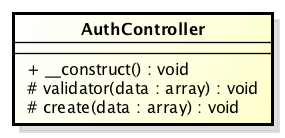
\includegraphics[width=0.5\linewidth]{img/back_end_http_controllers_authController}
\caption[Diagramma della classe AuthController]{Diagramma della classe AuthController}
\label{fig:back_end_http_controllers_authController}
\end{figure}
		\subparagraph{Descrizione}
			AuthController gestisce la registrazione dei nuovi utenti e i loro accessi.
		\subparagraph{Metodi}
			\begin{itemize}
				\item \textbf{+ \_\_construct()}\\
				Il costruttore della classe AuthController.
				\item \textbf{\# validator(data: array) : Validator}\\
				Il metodo si occupa della validazione di tutte le informazioni che riguardano l'utente al momento della registrazione.\\
					\textbf{Argomenti:}
						\begin{itemize}
							\item data : array;
							Array di valori contenente tutti i dati della registrazione di un utente. 
						\end{itemize}
				\item \textbf{\# create(data: array) : User}\\
				Il metodo si occupa della creazione di un nuovo utente:\\
					\textbf{Argomenti:}
						\begin{itemize}
							\item data : array;
							Array di valori contenente tutti i dati della registrazione di un utente.
						\end{itemize}
			\end{itemize}
		
\newpage
	\paragraph{PasswordController}
	\begin{figure}[h]
\centering
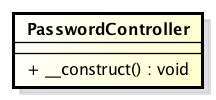
\includegraphics[width=0.5\linewidth]{img/back_end_http_controllers_passwordController}
\caption[Diagramma della classe PasswordController]{Diagramma della classe PasswordController}
\label{fig:back_end_http_controllers_passwordController}
\end{figure}

		\subparagraph{Descrizione}
			PasswordController contiene la logica per aiutare gli utenti per il reset delle loro credenziali di accesso.
		\subparagraph{Metodi}
			\begin{itemize}
				\item \textbf{+ \_\_construct()}\\
				Il costruttore della classe PasswordController.
			\end{itemize}
	
